\begin{figure}[htbp]
	\begin{minipage}{0.95\linewidth}
	\adjustbox{minipage=1.3em,valign=t}{\subcaption{}\label{fig:augds-a}}%
	\begin{subfigure}[t]{\dimexpr.5\linewidth-1.3em\relax}
		\centering
		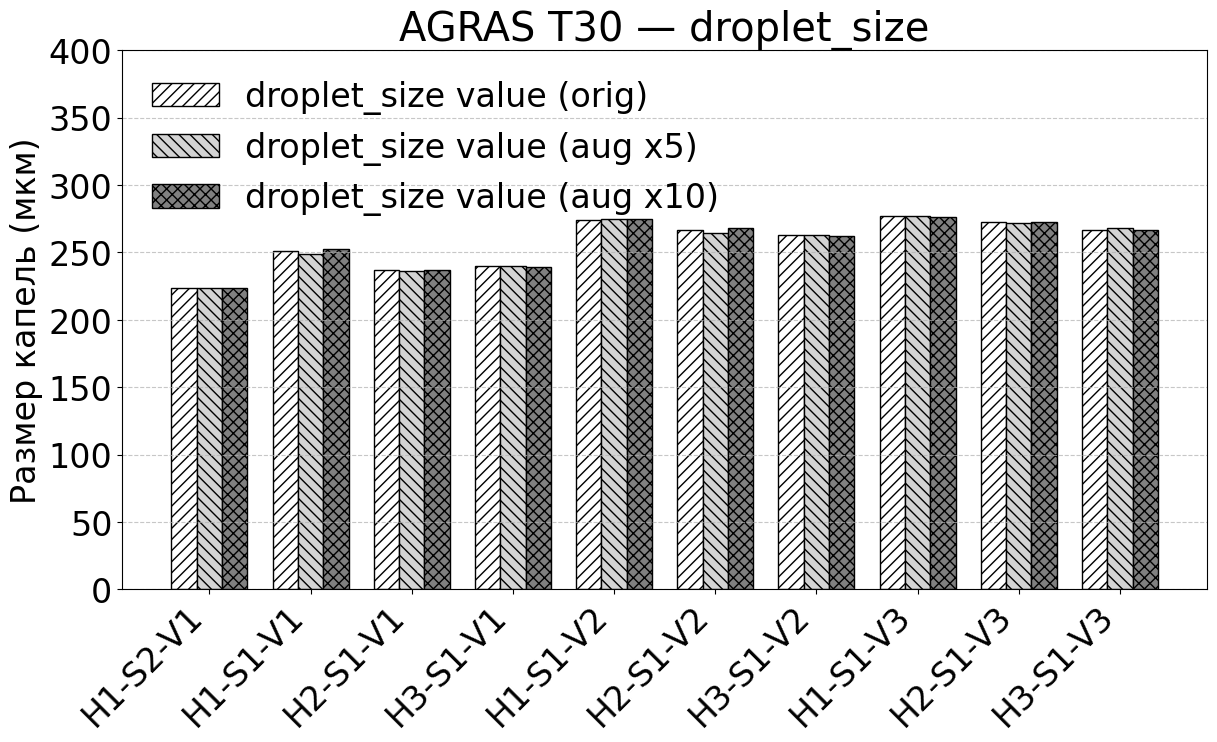
\includegraphics[width=.95\linewidth,valign=t]{my_folder/images/augment/spraying_performance/T30-droplet-size.png}
	\end{subfigure}
	\hfill %выровнять по ширине
	\adjustbox{minipage=1.3em,valign=t}{\subcaption{}\label{fig:augds-b}}%
	\begin{subfigure}[t]{\dimexpr.5\linewidth-1.3em\relax}
		\centering
		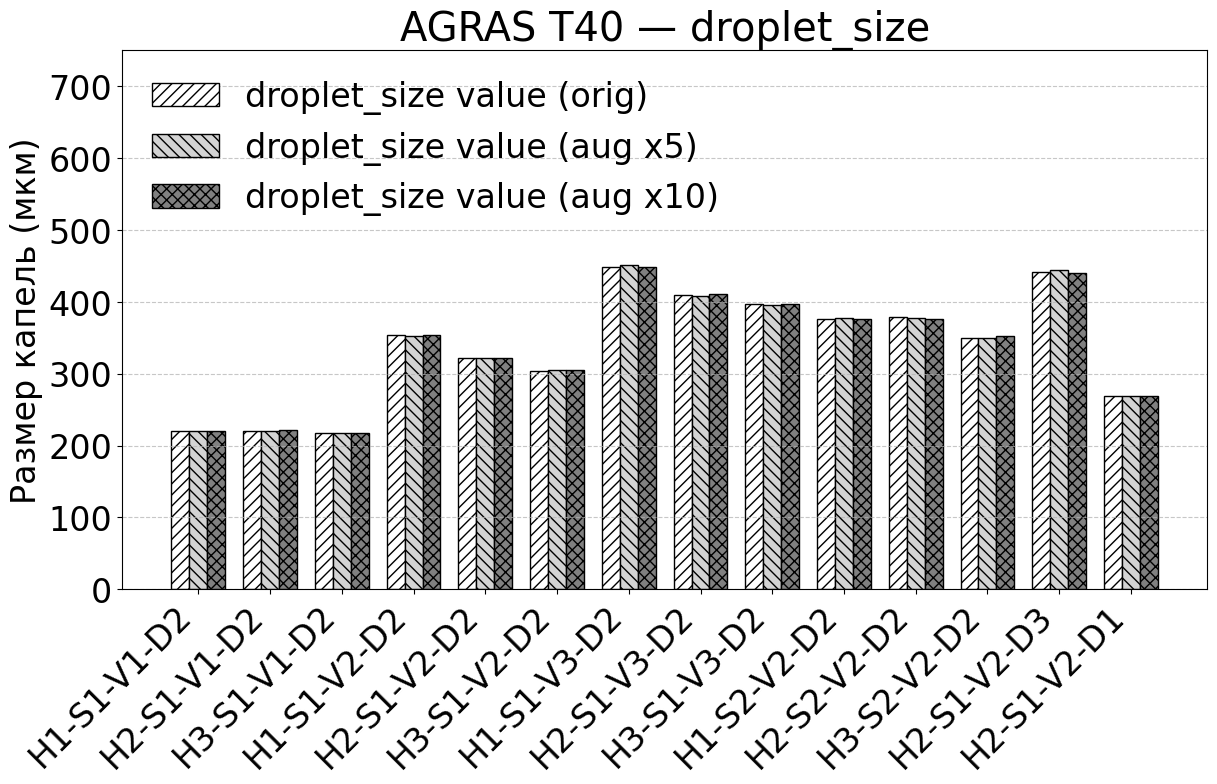
\includegraphics[width=.95\linewidth,valign=t]{my_folder/images/augment/spraying_performance/T40-droplet-size.png}
	\end{subfigure}
	\\[20pt]
	\adjustbox{minipage=1.3em,valign=t}{\subcaption{}\label{fig:augds-c}}%
	\begin{subfigure}[t]{\dimexpr.5\linewidth-1.3em\relax}
		\centering
		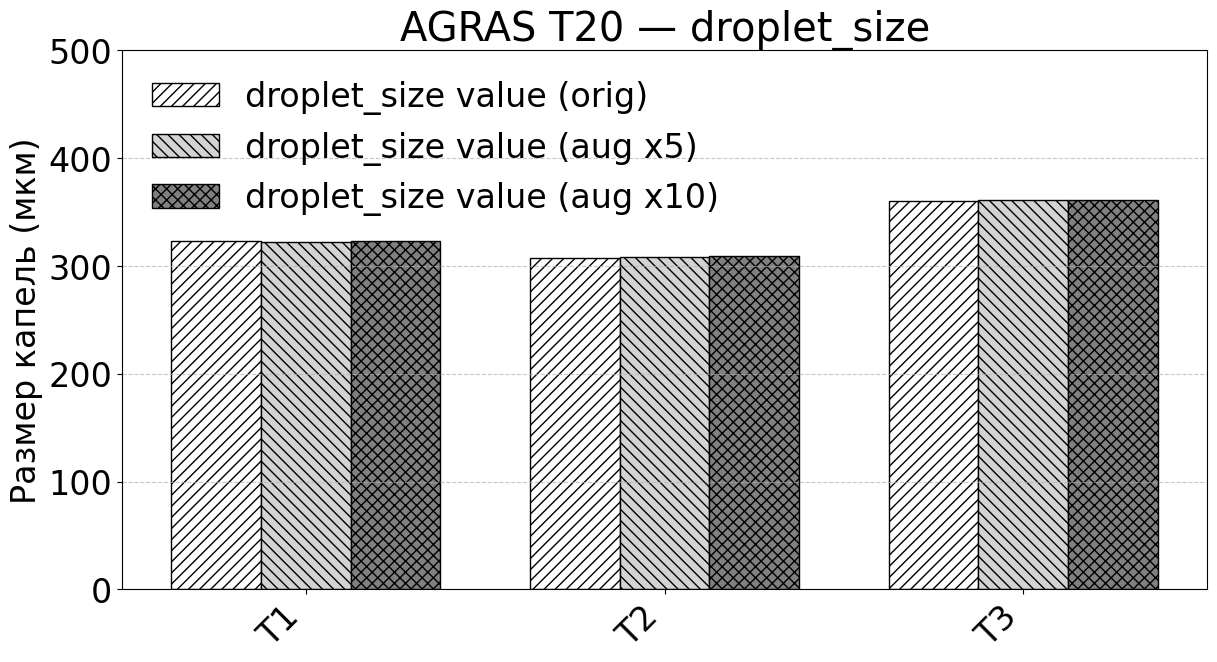
\includegraphics[width=.95\linewidth,valign=t]{my_folder/images/augment/droplet_deposition/T20-droplet-size.png}
	\end{subfigure}%
	\hfill %выровнять по ширине
	\adjustbox{minipage=1.3em,valign=t}{\subcaption{}\label{fig:augds-d}}%
	\begin{subfigure}[t]{\dimexpr.5\linewidth-1.3em\relax}
		\centering
		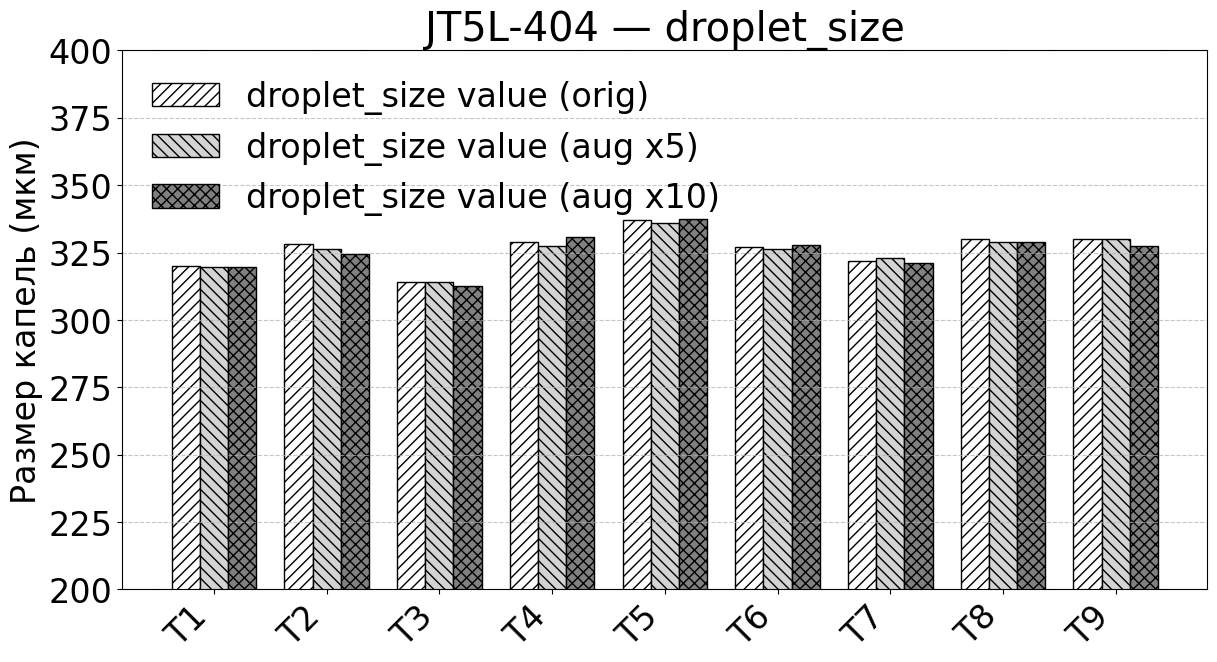
\includegraphics[width=.95\linewidth,valign=t]{my_folder/images/augment/coffee_science/JT5-droplet-size.png}
	\end{subfigure}
	\end{minipage}
	\captionsetup{justification=centering} %центрировать
	\caption{Распределение значений диаметра капель в исходной и аугментированных выборках: {\itshape a} --- AGRAS T30; {\itshape b} --- AGRAS T40; {\itshape c} --- AGRAS T20; {\itshape d} --- JT5L-404} 
	\label{fig:augment-droplet-size}
\end{figure}